\chapter{Gaussian and non-Gaussian random fields}\label{ch:random-fields}
\chapterstatus{written}{2026-11-14}

The initial conditions of a simulation, mock fields for testing estimators and the prior draws of field-level
inference all start from a realisation of a random field with a given power spectrum. This chapter describes how \fml{}
generates Gaussian fields on a grid, the two random-number backends (the N-GenIC-compatible line-seeded generator and
the counter-based Philox generator), amplitude-fixed and paired fields, and primordial non-Gaussianity of local,
equilateral, orthogonal and general quadratic form.

\begin{modulebox}{RandomFields and RandomGenerator}
\file{RandomFields/GaussianRandomField.h} (namespace \nsp{FML::RANDOM::GAUSSIAN}): white noise, Gaussian fields in
real and Fourier space, \cls{RandomFieldOptions} and the backends;
\file{RandomFields/CounterBasedRandomField.h} (Philox fields on any grid, e.g.\ \code{PencilGrid});
\file{RandomFields/NonLocalGaussianRandomField.h} (namespace \nsp{FML::RANDOM::NONLOCALGAUSSIAN}).\par
\file{RandomGenerator/RandomGenerator.h} (GSL and MT19937 generators), \file{RandomGenerator/CounterBasedRandom.h}
(Philox4x32-10).\par
Documentation: \file{RandomFields/README.md}, \file{SimulationCode/INITIAL_CONDITIONS.md}. Tests:
\file{tests/test_random_fields.cpp}.
\end{modulebox}

\section{Gaussian random fields on a grid}\label{sec:rf-gaussian}

A statistically homogeneous Gaussian field is fully described by its power spectrum. In a periodic box of side $B$
the Fourier modes $\delta(\vk)$, $\vk=2\pi\bm n/B$, are independent complex Gaussian variables with
$\langle|\delta(\vk)|^2\rangle=P(k)/V$, $V=B^N$, apart from the reality condition $\delta(-\vk)=\delta^*(\vk)$. With the
normalisation of \cls{FFTWGrid} (forward transform divided by $N_{\rm mesh}^N$, \cref{ch:conventions}) the grid
coefficients are drawn as
\begin{equation}
\delta_{\bm n}=\sqrt{\frac{P(k)}{V}}\;A_{\bm n}\,e^{i\theta_{\bm n}},\qquad
A_{\bm n}=\sqrt{-\ln U_1},\quad \theta_{\bm n}=2\pi U_2,
\label{eq:rf-mode}
\end{equation}
with $U_{1,2}$ uniform in $(0,1)$: a Rayleigh-distributed amplitude with $\langle A^2\rangle=1$ and a uniform phase,
equivalent to $(G_1+iG_2)/\sqrt2$ for two unit Gaussians. Only one of each pair $\{\vk,-\vk\}$ is drawn and the other
is its conjugate. The DC mode is zero, and the modes that are their own mirror image (the even-mesh Nyquist planes)
are handled by symmetry. The power spectrum is passed as a function \code{Pofk_of_kBox_over_volume}, $P(kB)/V$ of the
dimensionless wavenumber $kB$, so the generator itself is unit-free.

Fields can also be generated in real space: \code{generate_white_noise_field_real} draws unit Gaussian white noise
normalised to unit power (cell amplitude $N_{\rm mesh}^{N/2}$), which is Fourier transformed and multiplied by
$\sqrt{P(k)/V}$. This is the route of codes that start from a white-noise field, and makes it easy to impose
constraints in real space.

\paragraph*{Amplitude-fixed and paired fields.} With \code{fix_amplitude} only the phases are random,
$|\delta_{\bm n}|=\sqrt{P(k)/V}$ \cite{AnguloPontzen2016}. The field is then not Gaussian, but its power spectrum has no
sample variance mode by mode, and its statistics on the scales of interest are very close to those of Gaussian
fields \cite{VillaescusaNavarro2018}. With \code{reverse_phases} ($\theta\to\theta+\pi$) one obtains the pair of a
realisation; averaging the paired-fixed simulations cancels the leading-order (odd) contributions of the phases.
In SimulationCode: \param{ic_fix_amplitude} (default \code{true}) and \param{ic_reverse_phases}.

\section{Random number backends}\label{sec:rf-backends}

\paragraph*{N-GenIC (default).} \code{RandomFieldBackend::NGenIC} reproduces the generator of N-GenIC, 2LPTic,
L-PICOLA and MG-PICOLA: the random numbers are drawn line by line along the last dimension, with one seed per line
drawn from the supplied stateful generator (GSL or MT19937, \param{ic_random_generator}) and communicated so that the
result is independent of the number of MPI tasks and threads. A given seed therefore gives exactly the initial
conditions of those codes. The scheme has a known defect, kept for compatibility: the line seeds are
$\lfloor\code{INT_MAX}\cdot U\rfloor$, so there are only $\sim2^{31}$ of them and, by the birthday problem, about
$N_{\rm mesh}^{2N-2}/2^{32}$ lines get the same seed and perfectly correlated random numbers (13, 225 and 4136
duplicated lines for $N_{\rm mesh}=512$, 1024 and 2048 in 3D).

\paragraph*{Philox.} \code{RandomFieldBackend::Philox} uses the counter-based generator Philox4x32-10
\cite{Salmon2011}, implemented without external dependencies and checked against the integer known-answer vectors of
the Random123 repository. A counter-based generator is a keyed bijection: the random numbers of a mode are a pure
function of (key, counter), with no state. The 64-bit key is the seed; the 128-bit counter encodes the three signed
wave-vector coordinates injectively and a 32-bit \emph{stream} (an independent realisation or channel). The
representative of $\{\vk,-\vk\}$ is the one whose first nonzero coordinate is positive; the partner takes the
conjugate. Consequences:
\begin{itemize}
\item the value of a mode depends only on its wave vector, so the field is bit-identical for any number of MPI
      tasks, threads and any grid decomposition (\code{FFTWGrid} slabs, \code{PencilGrid}, \ldots);
\item the same seed gives the \emph{same} large-scale modes for any $N_{\rm mesh}$, so nested resolutions share their
      common modes (the power is evaluated directly at each mode, not interpolated, for this reason);
\item there are no seed collisions.
\end{itemize}
DC and even-mesh Nyquist planes are zero; odd meshes keep all modes. The uniforms are midpoint values strictly inside
$(0,1)$. All ranks must use the same seed, stream and power function, which must be callable concurrently with
OpenMP; non-finite or negative spectra are rejected. Integer outputs are portable; the Fourier coefficients may differ
in the last bits across platforms because of transcendental functions.

\begin{cppcode}[A Gaussian field with the Philox backend]
#include <FML/RandomFields/GaussianRandomField.h>
using namespace FML::RANDOM::GAUSSIAN;

FML::GRID::FFTWGrid<3> grid(Nmesh);
auto Pofk_of_kBox_over_volume = [&](double kBox) {      // P(k B)/V, k in 1/box
    double k = kBox / box;                               // h/Mpc
    return Pofk(k) / (box * box * box);
};
RandomFieldOptions options;
options.backend = RandomFieldBackend::Philox;
options.seed    = 1234;     // 64-bit key
options.stream  = 0;        // another realisation: another stream
generate_gaussian_random_field_fourier<3>(grid, nullptr, Pofk_of_kBox_over_volume,
                                          /*fix_amplitude=*/true, options);
\end{cppcode}

\begin{paramfile}[SimulationCode]
ic_random_field_backend = "philox"   -- default "ngenic": reproduces 2LPTic / L-PICOLA / MG-PICOLA
ic_random_seed          = 1234
ic_random_generator     = "GSL"      -- ngenic only: GSL or MT19937
ic_fix_amplitude        = true
ic_reverse_phases       = false
\end{paramfile}

\section{Primordial non-Gaussianity}\label{sec:rf-fnl}

Non-Gaussian initial conditions are generated in the primordial (Bardeen) potential $\phi$ as a quadratic
correction to a Gaussian field $\phi_G$,
\begin{equation}
\phi=\phi_G+f_{\rm NL}\,K[\phi_G,\phi_G],
\end{equation}
which gives a tree-level bispectrum $B_\phi(k_1,k_2,k_3)=2f_{\rm NL}[\,P_\phi(k_1)P_\phi(k_2)\,
\tilde K(\vk_1,\vk_2)+\text{perm.}]$. For the \emph{local} shape $K=\phi_G^2-\langle\phi_G^2\rangle$. For non-local
shapes, the method of Scoccimarro et al.\ \cite{Scoccimarro2012} writes the kernel in terms of fields filtered with
powers of the primordial spectrum, $\phi_\alpha\equiv P^{\alpha}\phi_G$ (a multiplication by $P(k)^\alpha$ in Fourier
space), so that every term is a product of two real-space fields and costs only FFTs:
\begin{equation}
K=c_0\left(\phi^2-\langle\phi^2\rangle\right)+c_1P^{1/3}\!\left[\phi\,\phi_{-1/3}\right]
+c_2P^{2/3}\!\left[\phi\,\phi_{-2/3}-\phi_{-1/3}^2\right]+c_3P\!\left[\phi\,\phi_{-1}-\phi_{-2/3}\phi_{-1/3}\right],
\label{eq:rf-kernel}
\end{equation}
with $\phi=\phi_G$ inside the brackets. The coefficients (\code{kernel_values}) are
\begin{center}\small
\begin{tabular}{@{}lcccc@{}}
\toprule
Shape & $c_0$ & $c_1$ & $c_2$ & $c_3$ \\
\midrule
local & $1$ & $0$ & $0$ & $0$ \\
equilateral & $-3(1-u)$ & $4-3u$ & $2$ & $-3u$ \\
orthogonal & $-9(1-u)$ & $10-9u$ & $8$ & $-9u$ \\
generic & \multicolumn{4}{c}{user supplied} \\
\bottomrule
\end{tabular}
\end{center}
where $u$ is the free parameter of the kernel family of Ref.~\cite{Scoccimarro2012} (the bispectrum does not depend on
it, the trispectrum and the scale-dependent bias do; $u=0$ by default).

\begin{implementation}[Implementation: non-local kernels]
The Gaussian $\phi_G$ is generated as unit white noise multiplied by $\sqrt{P(k)}$ evaluated exactly in every cell (a
cubic spline of the steep $k^{-3}$ primordial spectrum is inaccurate at low $k$ and can even go negative). Only the
filtered fields needed by the active terms are allocated and only the products that contribute are transformed: term 2
needs $\phi_{-1/3}$ even when $c_1=0$, term 3 needs $\phi_{-1/3}$ and $\phi_{-2/3}$. For the usual equilateral and
orthogonal shapes with $u=0$ this is five simultaneous grids and six transforms; at most six grids and eight
transforms. The DC mode is set to zero after each step and finished buffers are moved into the output. Kernel
parameters must agree on all ranks (the transforms are collective). The same \cls{RandomFieldOptions} select the
backend.
\end{implementation}

\paragraph*{Density field and conventions.}
\code{generate_nonlocal_gaussian_random_field_fourier_cosmology} generates $\phi$ with the primordial spectrum
$P_{\rm prim}(kB)/V=\frac{2\pi^2}{(kB)^3}A_s(k/k_{\rm pivot})^{n_s-1}$ and turns it into the density at the desired time
with the ratio $P_\delta(k)/P_{\rm prim}(k)$ (the transfer function and Poisson factor). The sign of $f_{\rm NL}$
depends on the sign convention relating the Bardeen and gravitational potentials. In SimulationCode
(\param{ic_random_field_type} \code{= nongaussian}, \param{ic_fnl_type}, \param{ic_fnl}) the non-Gaussianity is
added to $\Phi=\frac35g(z)\zeta$ at \param{ic_fnl_redshift}, with $g=D/a$ the linear suppression of the potential:
$z=0$ is the usual large-scale-structure convention and a matter-era redshift (e.g.\ 30) the CMB convention, with
$f_{\rm NL}^{\rm LSS}=f_{\rm NL}^{\rm CMB}/g(0)\approx1.27f_{\rm NL}^{\rm CMB}$ for $\Om_m=0.32$.

\begin{validation}[Validation (\file{tests/test_random_fields.cpp})]
\begin{itemize}
\item Philox: the zero, all-ones and $\pi$ known-answer vectors of Random123; DC/Nyquist and fixed-amplitude phase
      conventions in 2D and 3D; Hermitian symmetry through an FFT round trip ($2\times10^{-14}$); mean and power of the
      complex Gaussian samples; another stream gives another realisation; bit-identical output for different thread
      counts (and, per the module documentation, MPI decompositions); common Fourier modes identical across mesh
      resolutions.
\item N-GenIC: the explicit backend reproduces the legacy field and RNG state, and the GSL/2LPTic path.
\item Amplitude fixing gives $|\delta(\vk)|=\sqrt{P(k)/V}$ with the phases kept; \code{reverse_phases} gives
      $\delta(\vk)\to-\delta(\vk)$ exactly.
\item Non-Gaussian generator with $f_{\rm NL}=0$ reproduces the Gaussian field of the selected backend; SimulationCode's
      IC path dispatches to the selected backend and defaults to N-GenIC.
\end{itemize}
\end{validation}

\begin{figure}[htbp]
\centering
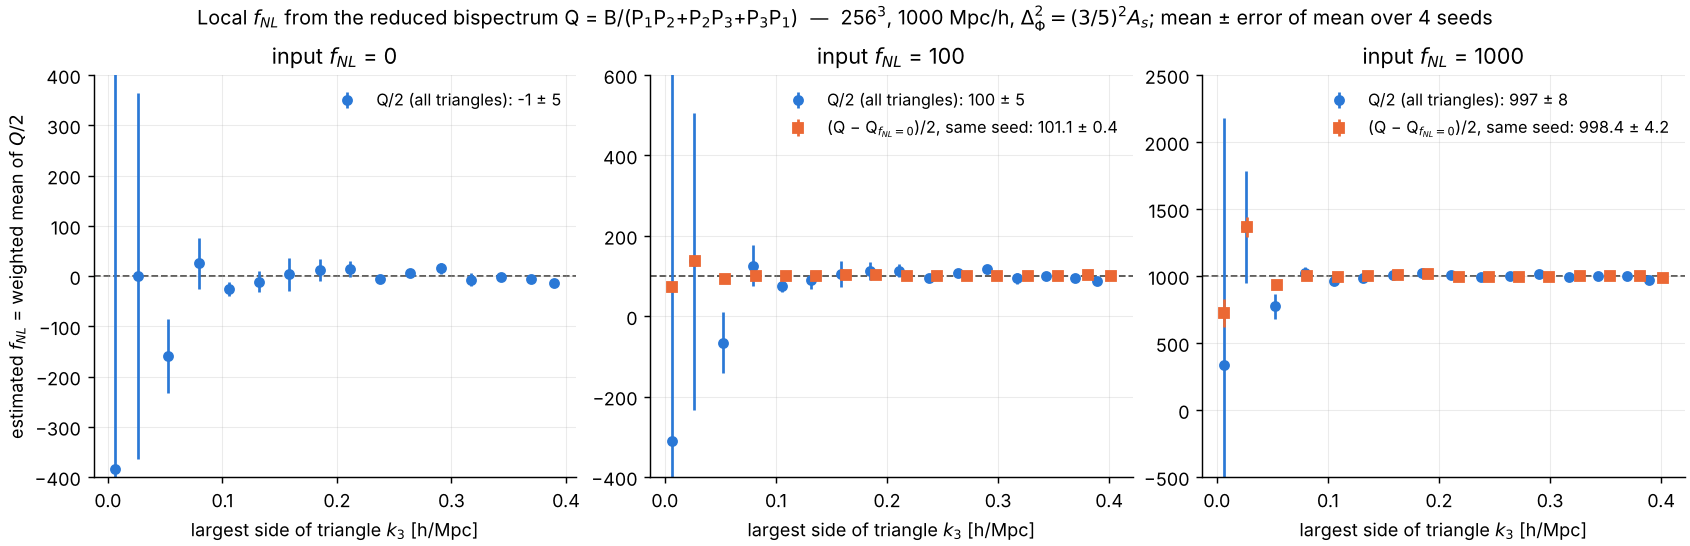
\includegraphics[width=\textwidth]{fnl_bispectrum}
\caption{Local $f_{\rm NL}$ recovered from the reduced bispectrum $Q=B/(P_1P_2+P_2P_3+P_3P_1)$ of non-Gaussian fields
($256^3$, $1000\Mpch$, mean and error over 4 seeds) for input $f_{\rm NL}=0$, 100 and 1000, as a function of the largest side of the
triangle. The same-seed difference $(Q-Q_{f_{\rm NL}=0})/2$ removes most of the cosmic variance of the Gaussian part. A standalone run
of \file{RandomFields} and \file{ComputePowerSpectra} with the method of \file{tests/test_fnl.cpp}.}
\label{fig:rf-fnl}
\end{figure}

